Este e un exemplo de artigo pa mostrar a estructura do repositorio.
Pode meterse simplemente con input.
A xente de edición debería coller os artigos do correos e editalos pa
que teñan un formato decente.

Logo metelos no documento principal é moi sinxelo, e versionar o codigo tamen.

\begin{enumerate}
    \item Engadir as citas
    \item Imaxes, con tamaños, posicións, resolucións, etc. adecuados
    \item Formato do texto vario e.g. \emph{enfatizado}
\end{enumerate}

\cite{VILABOA_apuntes.de.metodos.matematicos.2_2016}

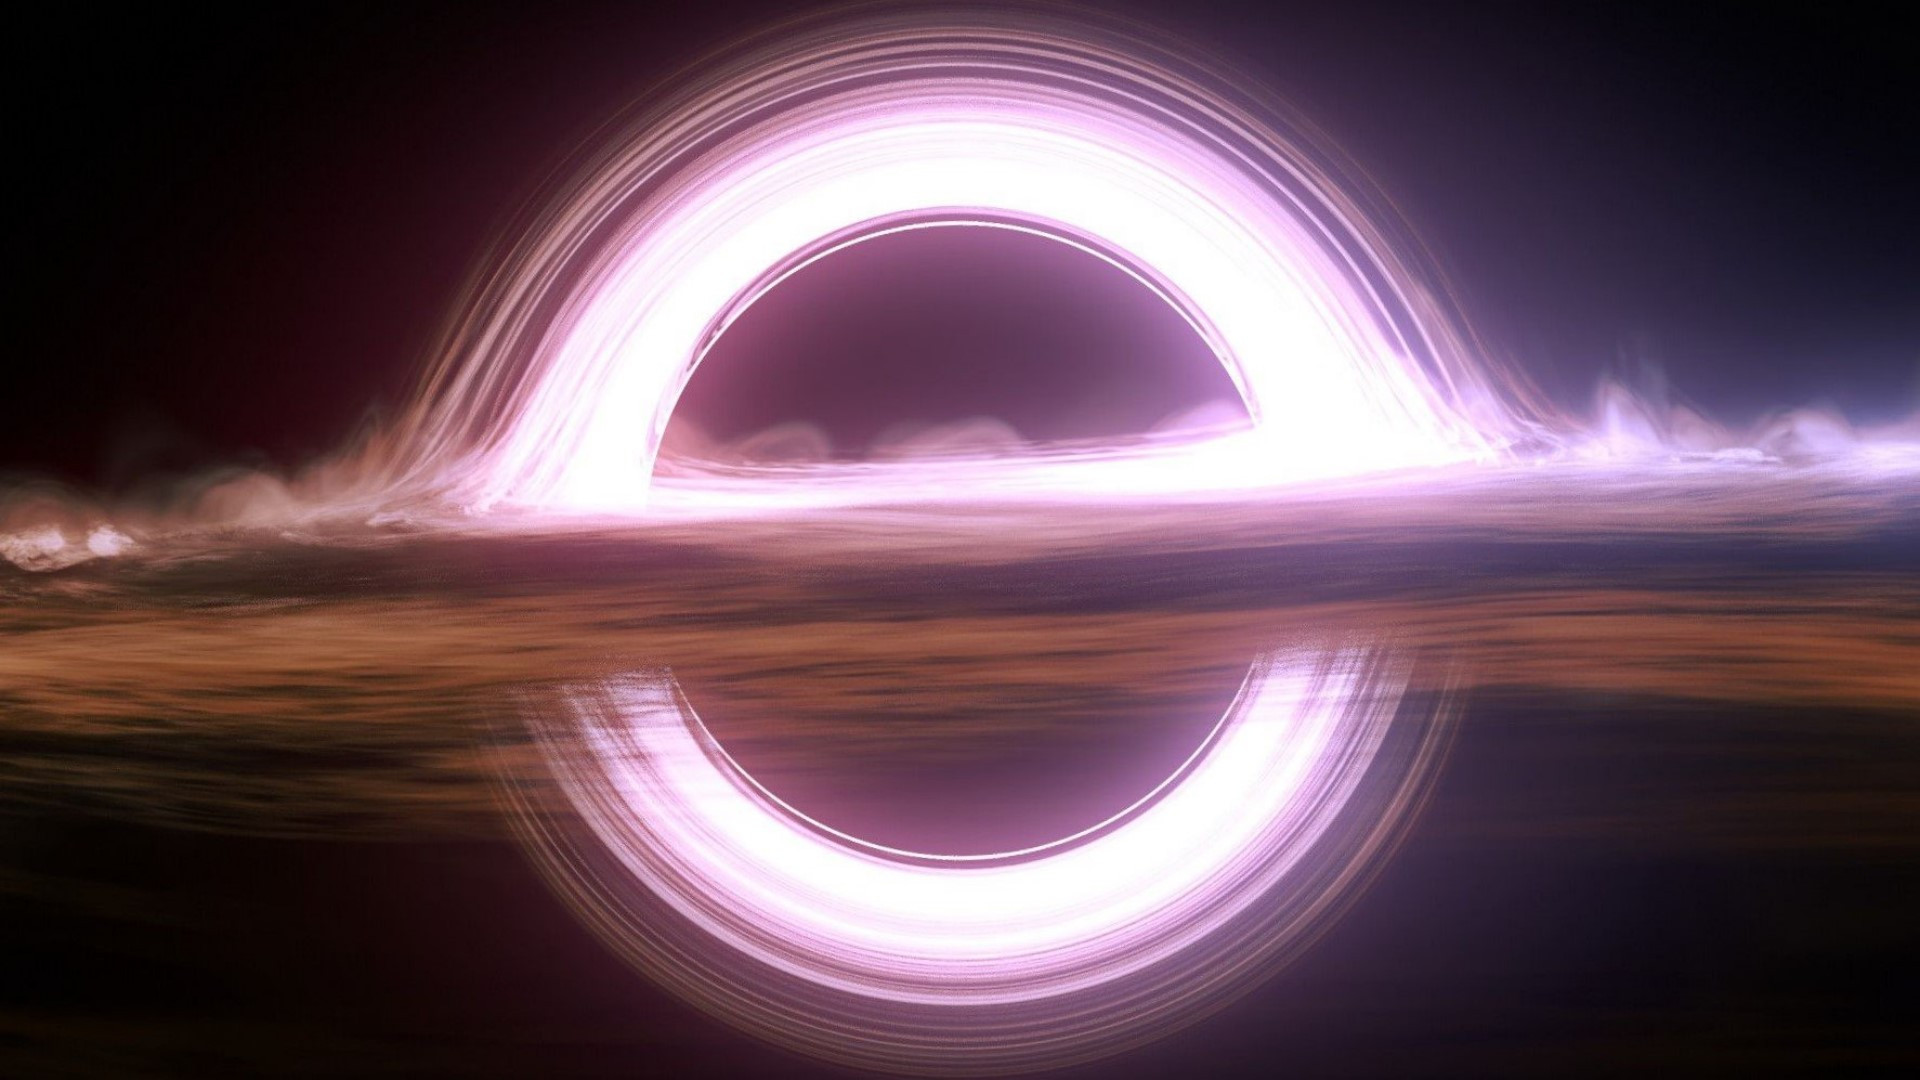
\includegraphics[width=\linewidth]{./revistas/001/imaxes/black_hole.jpg}

\lipsum
